
\begin{figure}[t]
    %\hspace{-10pt}
    \figuretitle{Fraction Reduction in PLT}
    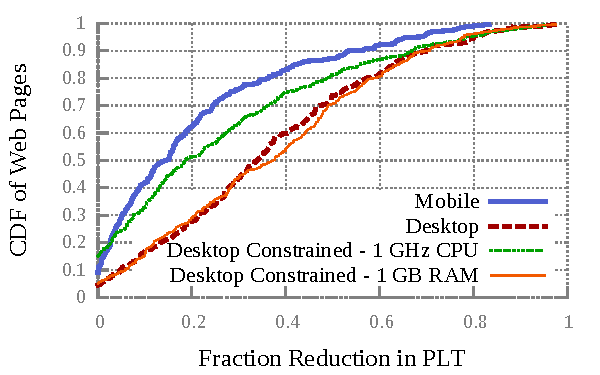
\includegraphics[width=3in]{../graphs/percent_plt_reduction/percent_reduction_linear.pdf}
    \caption[]{\label{fig:percent_reduction_linear}Reduction in page load time due to perfect caching is (significantly) less on mobile devices than desktop. When compared against two resource constrained VMs, CPU appears to be the deciding factor of the effectiveness of CDN caching.}
\end{figure}

% TODO(cs): this is fairly redundant with the abstract, and somewhat
% anti-climactic. For now, i'm going to try something with a bit more "punch";
% feel free to roll back though.
\eat{
We have presented an experimental apparatus for examining the effects of caching on mobile page load time.
We used this apparatus to extend the analysis done by Wang et
al.~\cite{wang2013demystifying}, which shows
that mobile page load time is not significantly improved by caching.
We developed a model to understand these effects, and our model indicates that
slow CPU speeds and low rates of caching on the critical path appear to be
the main cause of the difference between caching's effects on desktop versus mobile.
%Content providers may want to reconsider where they focus their optimization efforts, especially as mobile traffic begins to outpace its desktop counterpart.
}

Motivated by our initial surprise at Flywheel's weak performance improvements
from smarter caching, we sought to highlight and extend the analysis done by
Wang et al.~\cite{wang2013demystifying} which shows why caching should not
significantly improve page load time for mobile devices: slow CPU
speeds, and sparsity of cached (cacheable) items on the critical
path.

% TODO(cs): also a bit dry (potentially), although we should certainly add
% this back in if we have space.
% In future work we plan to measure the critical path on mobile devices, experiment with other web page load time metrics,
% and inflate the original network delays to better emulate mobile devices in congested network environments.

Going forward, mobile devices are becoming increasingly powerful, and the
bottleneck resources will shift. We hope that the model we have developed here
will help content providers and network designers make informed decisions about the performance
effects of caching for the mobile web of the future.

%\subsection{Future Work}
%There is still space to explore these findings. Using other metrics such as above-the-fold PLT and SpeedIndex may provide deeper insight into the reasoning behind limited mobile PLT reduction. Similarly, examining changes in the critical path with a tool such as WProf would provide valuable insight (WProf does not currently have a mobile tool). 

%It is also worth experimenting with varying levels of caching, namely 22\% and  32\% as in the Google NSDI paper~\cite{flywheel} to see if such incremental changes to mobile PLT are observed. \jamshed{Remove if done.}

%Finally, it is worth adding fixed delays to network responses in order to better emulate mobile and congested networks.
